\documentclass{article}
\usepackage{graphicx}
\usepackage[margin=1.5cm]{geometry}
\usepackage{amsmath}

\begin{document}
\twocolumn

\title{Friday Warm Up: Unit 6: Rotational Motion I}
\author{Prof. Jordan C. Hanson}

\maketitle

\section{Memory Bank}

\begin{itemize}
\item $s = r \theta$ ... Definition of the radian.
\item $\vec{s} = \vec{\theta} \times \vec{r}$ ... Vector relationship between angular displacement, arc length, and radius.
\item $v = r \omega$ ... Relationship between tangential velocity, angular velocity, and radius.
\item $\vec{v} = \vec{\omega} \times \vec{r}$ ... Vector relationship between tangential velocity, angular velocity, and radius.
\end{itemize}

\section{Rotational Variables and Rotational Motion}

\begin{enumerate}
\item A flywheel rotates such that it sweeps out an angle at the rate of 45.0 radians per second. The wheel rotates counterclockwise when viewed in the plane of the page. (a) What is the angular \textit{velocity} of the flywheel? (b) What direction is the angular velocity? (c) How many radians does the flywheel rotate through in 30 s? (d) What is the tangential speed of a point on the flywheel 10 cm from the axis of rotation? \\ \vspace{3cm}
\item Imagine the \textit{bolas} from previous warm ups.  Two point masses are rotating around a center of mass.  Let us determine the energy from the rotation.  (a) Write down the total kinetic energy in terms of the masses and the tangential velocities. (b) Substitute for the angular velocity using $v = r\omega$. (c) Factor the angular velocity squared.  What term remains?  What would this term be if there were three masses? (d) Let $I = \sum_i m_i r_i^2$. Show that the total kinetic energy is
\begin{equation}
K = \frac{1}{2}I \omega^2
\end{equation}
\end{enumerate}

\begin{figure}[hb]
\centering
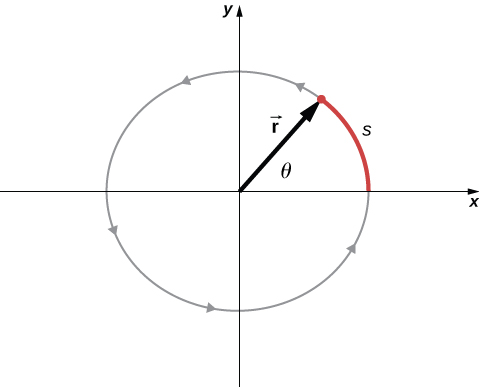
\includegraphics[width=0.45\textwidth]{figures/circle.jpeg}
\caption{\label{fig:1} Definition of the radian.}
\end{figure}

\begin{figure}[hb]
\centering
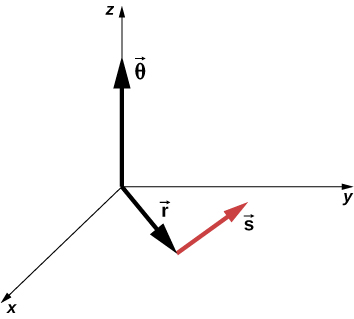
\includegraphics[width=0.4\textwidth]{figures/circle2.jpeg}
\caption{\label{fig:2} Vector relationship between angular displacement, arc length, and radius.}
\end{figure}

\end{document}
